\section{Client-Server Architecture}

The following section contains basic information about client-server architecture. At the 
end of the section, the group's own perspective will be shared along with the thoughts the 
group had in terms of this topic.

The client-server architecture is used as a way to distribute a system to other processors
which can be geographically spread\cite{ooad01}. An example of a client-server system is the 
credit card verification system implemented into each of a bank's terminals. This system 
verifies the credit card's authenticity with a centrally located server - in this case, each 
of a bank's terminals would be a client, and the central verification, would be the 
server\cite{ooad01}.

Illustrated, the client-server architecture looks as follows:

\begin{figure}[ht]
	\centering
		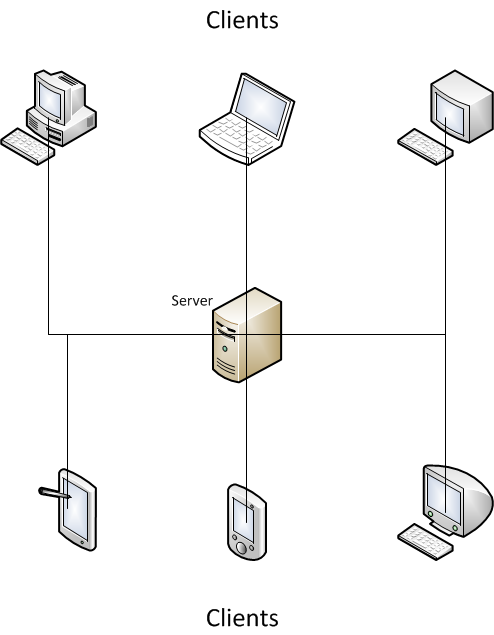
\includegraphics[scale=0.50]{design/figures/client-server.png}
	\label{fig:client-server architecture}
\end{figure}

The diagram is quite simplified and is by no means meant to illustrate an actual network. It
illustrates six clients: various forms of computers and some handheld devices all connected
to one, central server.


The purpose of the server is to offer to the clients whatever is general / common for each
client. This could be a common database, mail access, or some kind of printer  
functionality\cite{ooad01}. Basically, there are no restrictions. 


Client-server architecture can be more advanced than simply a client establishing a
connection to a server\cite{tierserverclient08}. These levels of advancement are called 
'tiers'\cite{tierserverclient08}. Tiers are the division of labour for various computer 
functions in a system.

\subsection{2-Tier Architecture}

2-tier architecture is quite simple. When a client has established a connection to a server, 
and begins to request resources, the server serves these in a response to the client. The 2-tier 
architecture does not make use of another application, because 
the server has access right away without needing an extra layer to give 
the client the resources requested\cite{tierserverclient08}.
\subsection{3-Tier Architecture}

3-tier architecture is slightly more advanced. The division of labour here is not 'simply' 
client / server. There is an extra layer - and for the sake of example this layer is a 
database server. This gives us the three layers of client, application server and database 
server. 


When the client requests data from the server, the server calls the database server, which 
sends an SQL query to the database to find this data. The database server then sends the 
fetched data to the application server, before sending it to the client in a response. This 
means that the client is linked to one server, and the server is linked to another server, 
which in turn is linked to a database\cite{tierserverclient08}.
\subsection{Tier 2 and 3 Compared}

The main thing to consider when comparing these two tiers is what characterizes them. Tier 2 
is obviously more versatile - it can handle all the requests it gets from the client without 
needing another layer. Tier 3 is less versatile, and much more 
specialized. The raw advantages of using tier 3 in the architecture, is the added security a server 
offers to a system. The added security is there because each part in the tier can define 
its own security measures. Multiple tiers offer better performance 
as well because tasks can be shared between the servers in the 
architecture\cite{tierserverclient08}.
\subsection{Our own perspective}

Given that the group has decided that scalability is a 'very important' non-functional 
requirement, making clever use of client-server architecture is a must for a final product. 
How it will be done in practice, is something to be considered for future work - given the 
scope of the program. 


The group recognizes that 2-Tier architecture would not be sufficient for this type of 
application. The program should be accessible through a browser, which means that the client 
should not have to install a program on their own machine to use our system. This also means 
that when the architecture is created, this should be kept in mind. A thin client is a 
client that does not need to process data locally - the processing should be on the server 
side\cite{thinclients08}. The servers will therefore be responsible for adding security 
layers to the system as mentioned in the 3-Tier architecture - but just as well the 
essential processing of the program.